\chapter{\acrshort{lid} Experiments}\label{Section: LID}

\todo{fill in Introduction sections.}

%###########################################################
%###########################################################
\section{Introduction}
%###########################################################
%###########################################################

\begin{itemize}
    \renewcommand\labelitemi{--}
    \item Look into computational model for babies LID
    \item Replication of idea introduced in Carbajal's thesis
    \item look into impact of bilingual background in LID
\end{itemize}


%%%%%%%%%%%%%%%%%%%%%%%%%%%%%%%%%%%%%%%%%%%%%%%%%%%%%%%%%%%%
\subsection{Motivations}

\begin{itemize}
    \renewcommand\labelitemi{--}
    \item Addition is regarding fully bilingual backgrounds
    \item Also aims at confirming the results with more ecological data 
\end{itemize}

%-----------------------------------------------------------
\subsubsection{Cognitive approaches}

% Overall cognitive approaches. No need to go too mych in details. 

\begin{itemize}
    \renewcommand\labelitemi{--}
    \item PRIMIR framework
    \item Possible to find experimental studies backing these results? Otherwise give it as motivation. 
    \item language filter hypothesis
\end{itemize}

%-----------------------------------------------------------
\subsubsection{Modelling approaches}
% Same as above

\begin{itemize}
    \renewcommand\labelitemi{--}
    \item ivectors
    \item show that embed well speaker characteristics
    \item idea that would akso 
    \item link with cogntive approaches. 
\end{itemize}

%###########################################################
%###########################################################
\section{Datasets}
%###########################################################
%###########################################################

%%%%%%%%%%%%%%%%%%%%%%%%%%%%%%%%%%%%%%%%%%%%%%%%%%%%%%%%%%%%
\subsection{Required characteristics}

\begin{itemize}
    \renewcommand\labelitemi{--}
    \item already had the xe dataset dewcribed Section x
    \item needed a matched dataset with clean data
    \item but also with bilingual speakers
    \item more description Section
\end{itemize}


% Need clean data on one side, ecological data on the other (see exp 2)
% replicating data from Julia
% also looking for bilingual datasets  (same people talking about both). Most important. 




%%%%%%%%%%%%%%%%%%%%%%%%%%%%%%%%%%%%%%%%%%%%%%%%%%%%%%%%%%%%
\subsection{\acrshort{ex} dataset} \label{Section: ex dataset}

\par The so-called \acrfull{ex} dataset corresponds to the train and test data used in \citet{carbajal2016language}. It is composed of two different languages using distinct continuous speech databases. American English utterances come from the \acrlong{timit} \citep{garofolo1993timit}, and the \acrlong{nchlt} \citep{barnard2014nchlt} was used to gather Xitsonga (a South-African language) speech. 

\par Three train sets were designed to match three background training conditions : two monolingual ones (English and Xitsonga) and a ``mixed" condition, consisting of a mix between English and Xitsonga utterances. All train sets were matched in duration, number of speakers and gender equity (see Table \ref{Table: Train Datasets XE}).

\par The test set is composed of 20 new speakers (half male half female), with matched number of utterances between the two languages, summing to a total of 200 utterances.

%FIND HOW GET TABLE AND CAPTION IN CENTER (not only table)
% Please add the following required packages to your document preamble:
% \usepackage{booktabs}
\begin{table}[h!]
\centering
\begin{tabular}{@{}lll@{}}
\toprule
Train set & \begin{tabular}[c]{@{}l@{}}N speakers\\ (\textit{N males})\end{tabular} & \begin{tabular}[c]{@{}l@{}}Duration\\ in minutes\end{tabular} \\ \midrule
English & \multicolumn{1}{r}{168 (84)} & \multicolumn{1}{r}{86.0} \\
Xitsonga & \multicolumn{1}{r}{168 (84)} & \multicolumn{1}{r}{87.0} \\
Mixed: & \multicolumn{1}{r}{168 (84)} & \multicolumn{1}{r}{87.9} \\
\multicolumn{1}{r}{\textit{English}} & \multicolumn{1}{r}{\textit{84 (42)}} & \multicolumn{1}{r}{\textit{43.7}} \\
\multicolumn{1}{r}{\textit{Xitsonga}} & \multicolumn{1}{r}{\textit{84( 42)}} & \multicolumn{1}{r}{\textit{44.2}} \\ \bottomrule
\end{tabular}
\captionsetup{justification=centering}
\caption{Summary of training sets in the \acrshort{ex} dataset. \\ Adaptation of Table 1 in \citet{carbajal2016language}.}
\label{Table: Train Datasets XE}
\end{table}



%%%%%%%%%%%%%%%%%%%%%%%%%%%%%%%%%%%%%%%%%%%%%%%%%%%%%%%%%%%%
\subsection{\acrshort{emime} dataset} \label{Section: emime dataset}

\par The \acrfull{emime} dataset \citep{wester2010emime} was chosen to carry out some of the bilingual experiments as it contains bilingual speech from the same bilingual speakers, allowing to create a``bilingual" train set beyond the monolingual and mixed sets described in Section \ref{Section: ex dataset}. 

\par The dataset is composed of English, Finnish and German speakers. For each of Finnish and German, the (native) speakers are also bilingual in English as well as being native in their own respective languages. There are 7 male and 7 female speakers in each language ($N=42$). 
\par The \acrshort{emime} dataset also has the advantage of offering for each speaker measures of accent rating in English. We decided to use the 2 best rated speakers of each language for the test sets, and the 5 other speakers for the train sets. 

%Talk about number of speakers in dataset. $


\bigskip

\par \noindent \textbf{\underline{Train sets.}}

\smallskip 

\par \noindent Eight train sets were created, fitting the three main training conditions described below:
\begin{itemize}[itemsep=2pt,topsep=4pt,itemindent=4pt]
    %\setlength\itemsep{0em}
    \renewcommand\labelitemi{$\ast$}
    \item \textbf{Monolingual}: Composed of a single language. 
        \begin{itemize}[itemsep=1pt,topsep=2pt]
        \renewcommand\labelitemi{--}
        \item \textbf{\textit{mono\_english\_native}} : English speech from native English speakers only.
        \item \textbf{\textit{mono\_english}} : English speech from native and non native English speakers. $\nicefrac{1}{3}$ of native English speakers, $\nicefrac{1}{3}$ of English speech from native German speakers and $\nicefrac{1}{3}$ of English speech from native Finnish speakers
        \item \textbf{\textit{mono\_german}} : German speech from native German speakers.
        \item \textbf{\textit{mono\_finnish}} : Finnish speech from native Finnish speakers.
        \end{itemize}
    \item \textbf{Mixed}: Mix between two languages. Each speaker in this condition is native and speaks only one of the two languages - there is no bilingual speaker. This corresponds to the mixed design in the \acrshort{ex} dataset. 
        \begin{itemize}[itemsep=1pt,topsep=2pt]
        \renewcommand\labelitemi{--}
        \item \textbf{\textit{mixed\_english\_german}} : $\nicefrac{1}{2}$ of English speech from native English speakers and $\nicefrac{1}{2}$ of German speech from native German speakers.
        \item \textbf{\textit{mixed\_english\_finnish}} : $\nicefrac{1}{2}$ of English speech from native English speakers and $\nicefrac{1}{2}$ of Finnish speech from native Finnish speakers.
        \end{itemize}
    \item \textbf{Bilingual}: This design is an addition compared to the train sets in the \acrshort{ex} dataset. It is composed of two languages, and each speakers in this design has utterances in both languages (\ie bilingual speakers). 
        \begin{itemize}[itemsep=1pt,topsep=2pt]
        \renewcommand\labelitemi{--}
        \item \textbf{\textit{bilingual\_english\_german}} : $\nicefrac{1}{2}$ of English speech from native German speakers and $\nicefrac{1}{2}$ of German speech from the same native German speakers.
        \item \textbf{\textit{bilingual\_english\_finnish}} : $\nicefrac{1}{2}$ of English speech from native Finnish speakers and $\nicefrac{1}{2}$ of Finnish speech from the same native Finnish speakers.
        \end{itemize}
\end{itemize}

Duration for each training set were matched to the \acrshort{ex} dataset to make the experiments as comparable as possible (see Table \ref{Table: Train Datasets EMIME}). 
 %TALK ABOUT THE PB WITH SENTENCES
\bigskip 


% Please add the following required packages to your document preamble:
% \usepackage{booktabs}
\begin{table}
\centering
\begin{tabular}{@{}lrr@{}}
\toprule
Background & \begin{tabular}[c]{@{}r@{}}N speakers\\ (N males)\end{tabular} & \begin{tabular}[c]{@{}r@{}}Total duration \\ in minutes\end{tabular} \\ \midrule
Mono English Native & 12 (6) & 87.0 \\
Mono English & 12 (6) & 87.0 \\
Mono German & 12 (6) & 87.1 \\
Mono Finnish & 12 (6) & 87.1 \\
Bilingual English German & 12 (6) & 87.5 \\
\multicolumn{1}{r}{\textit{English}} & \textit{6 (3)} & \textit{43.9} \\
\multicolumn{1}{r}{\textit{German}} & \textit{6 (3)} & \textit{43.6} \\
Bilingual English Finnish & 12 (6) & 87.2 \\
\multicolumn{1}{r}{\textit{English}} & \textit{6 (3)} & \textit{43.6} \\
\multicolumn{1}{r}{\textit{Finnish}} & \textit{6 (3)} & \textit{43.6} \\
Mixed English German & 24 (12) & 87.3 \\
\multicolumn{1}{r}{\textit{English}} & \textit{12 (6)} & \textit{43.6} \\
\multicolumn{1}{r}{\textit{German}} & \textit{12 (6)} & \textit{43.8} \\
Mixed English Finnish & 24 (12) & 87.2 \\
\multicolumn{1}{r}{\textit{English}} & \textit{12 (6)} & \textit{43.5} \\
\multicolumn{1}{r}{\textit{Finnish}} & \textit{12 (6)} & \textit{43.7} \\ \bottomrule
\end{tabular}
\captionsetup{justification=centering}
\caption{Summary of training sets in the \acrshort{emime} dataset}
\label{Table: Train Datasets EMIME}
\end{table}

\par \noindent \textbf{\underline{Test sets.}}

\smallskip

\par \noindent In addition, six test sets were created to fit the three test designs. All test sets have the same number of utterances as the test set in the \acrshort{ex} dataset ($N=200$), 100 per language (all different sentences), with equal gender distribution. The average utterance duration was of 3.86 seconds. The speakers were, for each language and gender, those with the highest accent rating. :
\begin{itemize}[itemsep=2pt,topsep=4pt,itemindent=4pt]
    %\setlength\itemsep{0em}
    \renewcommand\labelitemi{$\ast$}
    \item \textbf{Monolingual}: It has a different meaning as in the train design. It is composed of a mix of two languages, each speaker being native in each language,there is no speaker overlap between the languages:
        \begin{itemize}[itemsep=1pt,topsep=2pt]
        \renewcommand\labelitemi{--}
        \item \textbf{\textit{mono\_english\_german}} : $\nicefrac{1}{2}$ of English speech from native English speakers and $\nicefrac{1}{2}$ of German speech from native German speakers ($N\_speakers=4$).
        \item \textbf{\textit{mono\_english\_german}} : English speech from native English speakers and Finnish speech from native Finnish speakers ($N\_speakers=4$). 
        \end{itemize}
    \item \textbf{Bilingual}: The meaning is also different from the training sets' one. Mix between two languages. Each speaker in this condition is native and speaks only one of the two languages - there is no bilingual speaker. This corresponds to the mixed design in the \acrshort{ex} dataset. 
        \begin{itemize}[itemsep=1pt,topsep=2pt]
        \renewcommand\labelitemi{--}
        \item \textbf{\textit{mixed\_english\_german}} : $\nicefrac{1}{2}$ of English speech from native German speakers and $\nicefrac{1}{2}$ of German speech from the same native German speakers ($N\_speakers=4$). 
        \item \textbf{\textit{mixed\_english\_finnish}} : $\nicefrac{1}{2}$ of English speech from native Finnish speakers and $\nicefrac{1}{2}$ of Finnish speech from the same native Finnish speakers ($N\_speakers=4$).
        \end{itemize}
    \item \textbf{Mixed}: Different meaning from from the mixed train set. It is a combination of the ``monolingual" and ``bilingual" test designs. 
        \begin{itemize}[itemsep=1pt,topsep=2pt]
        \renewcommand\labelitemi{--}
        \item \textbf{\textit{bilingual\_english\_german}} : $\nicefrac{1}{4}$ of English speech from native English speakers, $\nicefrac{1}{4}$ of English speech from native German speakers (different sentences) and $\nicefrac{1}{2}$ of German speech from the same native German speakers ($N\_speakers=4$).
        \item \textbf{\textit{bilingual\_english\_finnish}} : $\nicefrac{1}{4}$ of English speech from native English speakers, $\nicefrac{1}{4}$ of English speech from native Finnish speakers (different sentences) and $\nicefrac{1}{2}$ of Finnish speech from the same native Finnish speakers ($N\_speakers=4$).
        \end{itemize}
\end{itemize}

\bigskip

\par \noindent \danger \hspace{0.1cm} \textbf{Sentences repetitions.} Because of the relatively small size of the dataset, the sentences in the test set also exist in the training set, albeit with different speakers. Moreover, sentences in the training set appear multiple time, spoken by different speakers.  This poses a serious issue as it means that the i-vectors  - or other speech representations - in posterior experiments might capture the pattern of the sentences itself rather than other sought for characteristics as language or speaker specific features. It could thus invalidate some of the results because of the repetitions between the training and test sets. A ``spontaneous speech" dataset could solve this issue but it is really hard to find one with bilingual speakers. On the other hand, one could argue that this kind of setup might be closer to what young children encounter in their environment, with a high frequency effect \textit{... need references}
%eg of studies on frequencies https://files.eric.ed.gov/fulltext/EJ1141442.pdf

\bigskip

Another major difference between the two datasets, besides the sentences repetition, is the number of speakers. The \acrshort{emime} dataset has significantly less speakers than the \acrshort{emime} dataset. However, the same argument as the sentences repetition issue can be held here, making the data maybe slightly more ecological: young children tend to have a small number of speakers in their environment \textit{... need references}.
% Explain how for each experiment it's either englosh finnish or english german


                                       
%%%%%%%%%%%%%%%%%%%%%%%%%%%%%%%%%%%%%%%%%%%%%%%%%%%%%%%%%%%%
\subsection{Other datasets to consider}
[...]


%###########################################################
%###########################################################
% \section{Impact of bilingual background in \acrshort{lid}}
\section{Impact of multilingual environment in LID}
 \hspace{0.65cm}{\large\textit{Replication of \citet{carbajal2016language}}}\label{Section: impact of multilingual in lid}
%###########################################################
%###########################################################

\bigskip

In this section, we aim to replicate the pipeline and results presented in \citep{carbajal2016language}. The same dataset as in the publication was used, described in  Section \ref{Section: ex dataset}. 

\bigskip
\todo{Give some info on the results found by Julia (will be detailed in the discussion section). Also give original hypotheses.}


%Explain that replication of Julia

%%%%%%%%%%%%%%%%%%%%%%%%%%%%%%%%%%%%%%%%%%%%%%%%%%%%%%%%%%%%
\subsection{Methods}\label{Section: replication pipeline}

We tried to reproduce the pipeline in \citet{carbajal2016language} as close as possible.  However, we used slightly different tools, meaning some of the parameters were somewhat different. 

The original pipeline consists in extracting \acrfull{mfcc} from the speech, training a full \acrfull{ubm}, deriving a \acrfull{tvs} and extracting I-Vectors. More information on the exact pipeline are given in \citet{carbajal2016language}. In some variations of the experiments, we also carried out a \acrfull{lda} based on speakers labels, either on the train or on the test I-vectors \textbf{\textit{(more explanation below)}}. 

Although the parameters were kept the same as in \citet{carbajal2016language}, the main different lies in the tools used. We used the open-source toolkit Kaldi \citep{Povey_ASRU2011} for the whole pipeline (features extraction, \acrshort{ubm} training, I-Vectors extraction), and the code can be found on the \href{https://gitlab.coml.lscp.ens.fr/mde/lid.git}{team Github repository}\footnote{access has to be asked directly to the repository owner}.

\bigskip
\todo{Insert more info on pipeline details + details on how the UBM differ}

\bigskip
\todo{Detail ABX measure and link to section below}



%%%%%%%%%%%%%%%%%%%%%%%%%%%%%%%%%%%%%%%%%%%%%%%%%%%%%%%%%%%%
%\subsection{Some caveats of the original experiment}
\subsection{Suggested improvements on the original experiment}\label{Section: improvement on carbajal}


Some methods used in the original experiment in \citet{carbajal2016language} are worth reconsidering, as they might not be the best approaches to validate the original hypotheses. 

\bigskip 

\par \noindent \textbf{LDA analysis.} In the original experiment, speaker-based \acrshort{lda} was carried out on the test I-vectors to maximise the distance between speakers, as a mean to investigate the role of speaker information on language separation. However, applying \acrshort{lda} to the test I-Vectors means we basically directly give out all of the speaker information we have on the test speakers, which can't be a good computational model of \acrshort{lid} acquisition. It is indeed hardly surprising that the \acrshort{lid} scores are extremely high if they are computed on i-vectors which are speaker separated especially when in the test set, speakers only speak either one or the other language. It can't be  a good computational model of \acrshort{lid} acquisition, as children wouldn't normally have this speaker information readily available, neither in an ecological environment nor in experimental settings. The idea to apply \acrshort{lda} to i-vectors was nevertheless an interesting idea, as it is possible that speakers make use of speaker-dependent features that they have previously learned to process \acrshort{lid}. 

\bigskip 

\par \noindent \textbf{ABX measures.} The ABX discrimination score (ref) was used as prime measure of \acrshort{lid} \citep{schatz2013evaluating}. This measure, based on the experimental psychology counterpart, allows for computing the extent to which within category distances are smaller than between category distances. The details are further explained in \citet{carbajal2016language}, but in short, it consist in computing distances between ``triplets" of representations (here the speech segments' i-vectors) where two representations are from the same category and one is from the other category, and compute if the model representations correctly categorises which ones are from the same category.  
%Careful - plagiarised end of sentence from julia. 
With this method, it is usually possible to control for independent variables by only using specific subsets of all the possible triplets (using the so-called ``across" and ``by" options. However, in the experiment's specific design, there is no straightforward way to control for the ``speaker" variable using the main available options. In \citet{carbajal2016language}, there is no proper control of this variable, leading to triplets where the two within-category representations share the same feature \footnote{the ``across" option can't be used here as there are no bilingual speakers, and thus no between-category pairs with the same speaker.} Not controlling for this method means the distance between the representations can be highly biased by the speaker information, as a possible reason for the within-category pairs to be closer would be because of the speaker features. We argue that a fairer measure would discard possible within-category pairs where the speaker is the same. This was done in further experiments using the ``filter" option available in the \href{https://github.com/bootphon/ABXpy}{ABXpy toolkit} \textbf{and is referred to as... X ...}. 

%Give the name used for filtered
%explain train ivectors. /

%%%%%%%%%%%%%%%%%%%%%%%%%%%%%%%%%%%%%%%%%%%%%%%%%%%%%%%%%%%%
\subsection{Original Results}

ABX results and \acrfull{mds} plots on the different training conditions from \citet{carbajal2016language} are presented \ref{Table: ABX score Julia Exp} and Figure \ref{Figure: Julia MDS}.

First of all, the monolingual backgrounds results suggest that utterances are relevant for \acrshort{lid} and that they can be computationally modelled by Gaussian mixtures - yielding high language discrimination scores (similar to experimental results?). This suggests the pipeline is a reasonable model of processing for how infants undertake language discrimination tasks, providing that they have been exposed prior to a minimum amount of (at least monolingual) data - experience which is modelled by the \acrshort{ubm}).

\bigskip

One of the main findings is that ``mixed" backgrounds yielded lower ABX scores than its monolingual counterparts, suggesting - if the process is a good model of how infants learn to discriminate languages - that children having been exposed to mixed speech would find the \acrshort{lid} task more difficult. \textbf{To our knowledge, no cognitive experiments were carried out to investigate this hypothesis? (and pretty hard to measure infants prior exposure to mixed/bilingual speech. } This finding was not however extensively discussed in \citet{carbajal2016language}, and we would like to raise the important point of ecological validity of the ``mixed" train set - as it is very unlikely for an infant to be exposed to equal amount of speech of two languages.

\bigskip

\par Another important point raised is that \acrshort{lda} strongly improved the ABX scores, and particularly when the background is mixed. \citet{carbajal2016language} present it as potential evidence for the idea that infants uses some non-linguistic cues (here speaker information) to discriminate languages. However, as discussed in Section \ref{Section: improvement on carbajal}, carrying out the \acrshort{lda} on the test i-vectors probably isn't an accurate method as it does not model the \acrshort{lid} process.  This can be further verified looking at the \acrshort{mds} plots in Figure \ref{Figure: Julia MDS}, where the speech representations seem to be strongly grouped per speaker. This doesn't mean the conclusions are incorrect but more valid methods are required to validate this hypothesis. In the replication results below, we present results where \acrshort{lda} is carried out on the train i-vectors. 
Another discus
For more details and further discussion, refer to \citet{carbajal2016language}.

\bigskip
Three caveats are also raised in the article. First, the pipeline implies that exposure to language is required to perform \acrshort{lid}, but results show that infants can discriminate languages from their first day , suggesting that accumulation of data is done continuously (?). There is also the problem, already mentioned, of ecological validity of the dataset - which contains a high number of speakers, and - in the case of the mixed dataset, where there are no bilingual speakers. This problem is solved with the \acrshort{ex} dataset. Finally, only static features were used in this experiment, where dynamic information could possibly be of use. We also experiment this in Section \ref{Section: julia rep dynamic}.  


%Need to keep in mind the caveats found in Section X,.....
\bigskip

% Please add the following required packages to your document preamble:
% \usepackage{booktabs}
% \usepackage{multirow}
\begin{table}[h!]
\centering
\begin{tabular}{@{}lcc@{}}
\toprule
\multirow{2}{*}{Background} & \multicolumn{2}{c}{ABX score} \\
 & pre-LDA & \begin{tabular}[c]{@{}c@{}}post-LDA\\ (on test i-vectors)\end{tabular} \\ \midrule
English & 72.8 & 90.7 \\
Xitsonga & 69.8 & 92.1 \\
Mixed & 54.3 & 82.1 \\ \bottomrule
\end{tabular}
%\captionsetup{justification=centering}
\caption{Summary of ABX results (in \% correct) in the original experiment. Adapted from \citet{carbajal2016language}. }
\label{Table: ABX score Julia Exp}
\end{table}

\begin{figure}[h!]
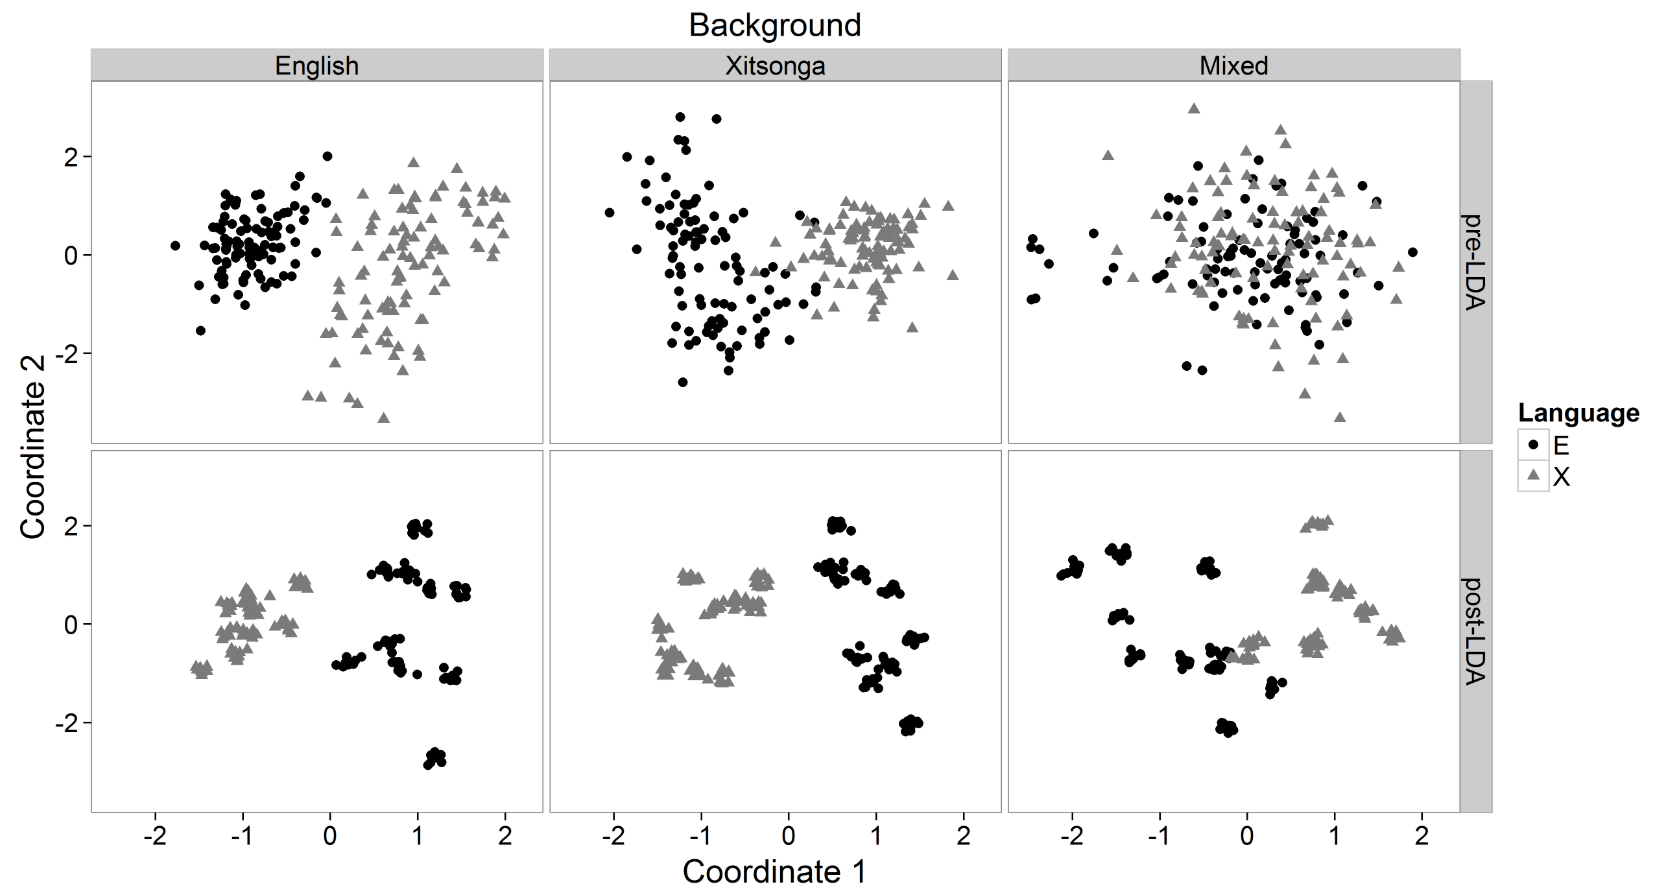
\includegraphics[width=\textwidth, height=\textheight,keepaspectratio]{julia_mds.png}
\caption{Multidimensional Scaling plot of English (black dots) and Xitsonga (grey triangles) test utterances for three different language backgrounds (English, Xitsonga or mixed), pre- and post-LDA (top and bottom rows, respectively). Adapted from \citet{carbajal2016language}.}
\label{Figure: Julia MDS}
\end{figure}


\bigskip
%key points
\par \noindent \fbox{\parbox{\textwidth}{
\begin{itemize}[leftmargin=*]
    \setlength\itemsep{0em}
    %\renewcommand\labelitemi{$\circ$}
    \item \textbf{Mixed background yields worst results than monolingual backgrounds, pre- and post-LDA}
    \item \textbf{LDA on test set strongly improves abx scores, especially with mixed background}
    \item \textbf{LDA on test i-vectors probably isn't a valid method}
\end{itemize}}}



%%%%%%%%%%%%%%%%%%%%%%%%%%%%%%%%%%%%%%%%%%%%%%%%%%%%%%%%%%%%
\subsection{Replication Results} \label{Section: julia rep results}


The experiment in \citet{carbajal2016language} was replicated using the pipeline described in Section \ref{Section: replication pipeline} (as explained before, the train and test sets are the same, however the tools used for the different tasks (feature extraction, \acrshort{ubm} training, i-vectors extractions and abx scoring) differ as the toolkits used are different. 
\bigskip

Results are reported in Table \ref{Table: ABX score Julia Rep} and the \acrshort{mds} plots in Figure \ref{Figure: Julia Replication MDS}. Although the scores differ between the original and the replication experiments, we can identify the same patterns : monolingual training backgrounds tend to yield higher abx scores than mixed backgrounds, and \acrshort{lda}  on the test-i-vectors significantly improves the scores (especially for the mixed background). However as discussed before, carrying out \acrshort{lda} on the test i-vectors isn't predictor of a strong model. 
\par We also computed the abx scores by filtering out the "within-pair" doublons with identical speaker, as discussed in Section \ref{Section: improvement on carbajal}. Although as expected, this leads to lower scores, the patterns don't change. 


% Please add the following required packages to your document preamble:
% \usepackage{multirow}
\begin{table}[h!]
\centering
\begin{tabular}{lcc}
\hline
\multirow{2}{*}{Background} & \multicolumn{2}{c}{ABX score} \\
 & pre-LDA & \begin{tabular}[c]{@{}c@{}}post-LDA\\ (on test i-vectors)\end{tabular} \\ \hline
English & 75.6 \textit{(73.2)} & 95.5 \textit{(95.1)} \\
Xitsonga & 79.5 \textit{(77.6)} & 98.1 \textit{(97.9)} \\
Mixed & 65.2 \textit{(61.8)} & 85.2 \textit{(83.7)} \\ \hline
\end{tabular}
\caption{Summary of ABX results (in \% correct) in the replication of \citet{carbajal2016language}'s experiment. The abx scores in italics as those obtained when excluding with the same speaker in the within-class pair. }
\label{Table: ABX score Julia Rep}
\end{table}



\par An interesting difference can be noted when analysing the \acrshort{mds} plots. In \citet{carbajal2016language}' plots, it seemed that, for monolingual backgrounds, the "original language" would form a denser cloud than the new language, which could be explained by the larger amount of information on this specific language in the \acrshort{ubm}, making it easier to gather the utterances. 

\begin{figure}[h!]
\fbox{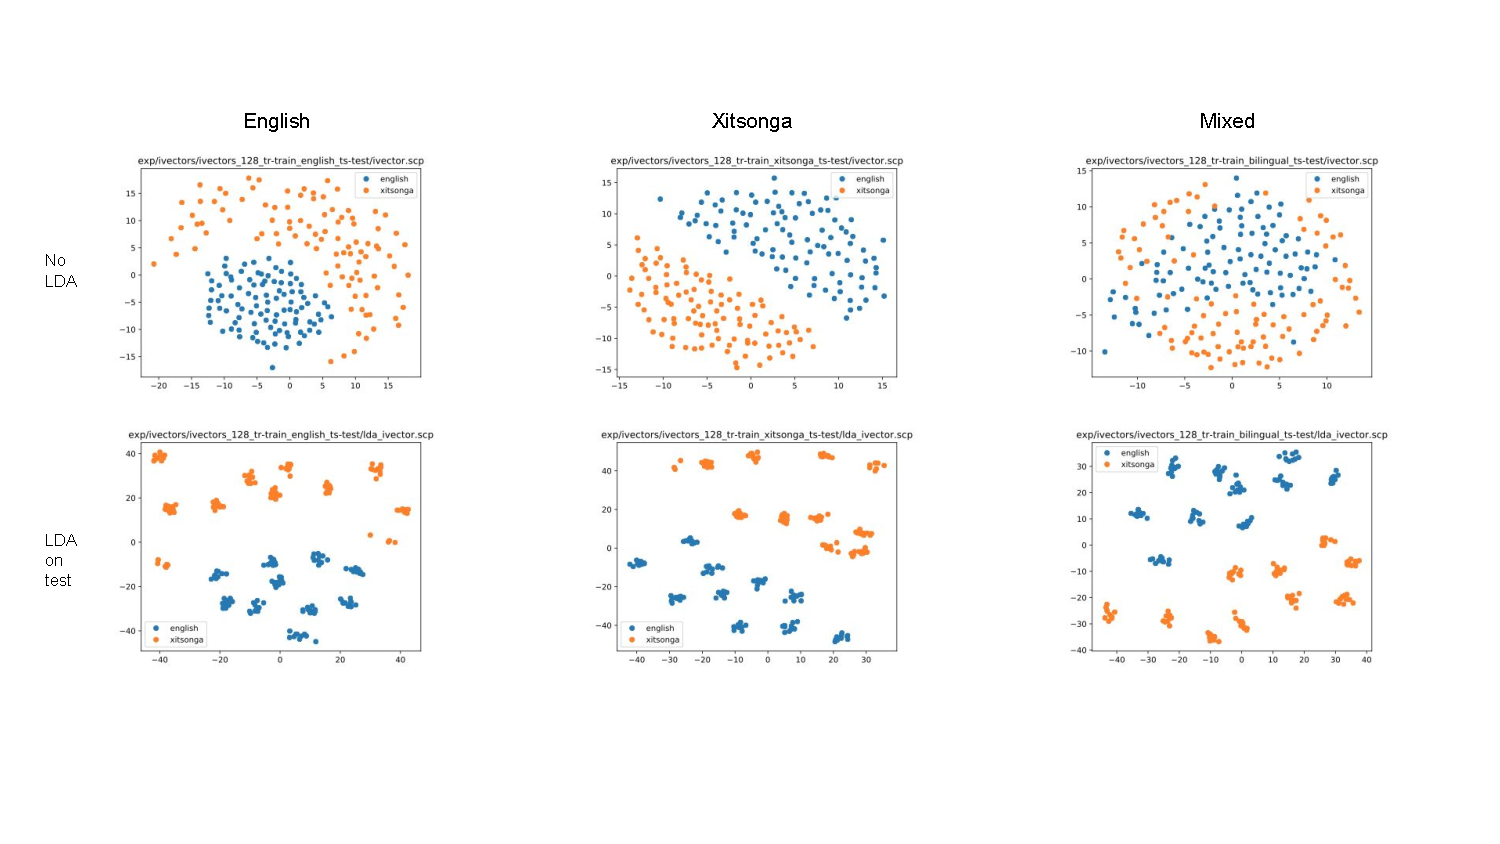
\includegraphics[width=\textwidth, height=\textheight,keepaspectratio,trim={0 2.5cm 1cm 1.5cm},clip]{julia_replication_mds.pdf}}
\caption{Multidimensional Scaling plot of English (blue) and Xitsonga (orange) test utterances for three different language backgrounds (English, Xitsonga and Mixed), pre-LDA and post-LDA on test i-vectors (top and bottom rows respectively); for the replication results of \citet{carbajal2016language} experiment.}
\label{Figure: Julia Replication MDS}
\end{figure}
\bigskip 
\todo{improve figure drastically}

\bigskip
%key points
\par \noindent \fbox{\parbox{\textwidth}{
\begin{itemize}[leftmargin=*]
    \setlength\itemsep{0em}
    %\renewcommand\labelitemi{$\circ$}
    \item \textbf{Similar patterns to original experiment, even with the corrected abx measure.}
    \item \textbf{Difference in that in monolingual background, not necessarily a denser cloud for the original language in the \acrshort{mds} plot.}
\end{itemize}}}


%%%%%%%%%%%%%%%%%%%%%%%%%%%%%%%%%%%%%%%%%%%%%%%%%%%%%%%%%%%%

\subsection{\acrshort{lda} on train ivectors} \label{Section: Julia rep exp - lda}

As discussed in Section \ref{Section: improvement on carbajal}, we argue that it would be more valid to compute the \acrshort{lda} on the train i-vectors rather than on the test ones, as it would correspond to gathering speaker information on the already seen data (speech the infant was exposed to prior to the test), and then make use of this learnt information to try to discriminate the novel test data. To compute \acrshort{lda}, we need to use $N\_Speakers$\textit{-1} dimensions. However, because the i-vectors dimensions (150) is in the original experiment smaller than the required \acrshort{lda} dimensions (167), we decided to change the i-vectors dimension to 200, in order to investigate the role \acrshort{lda} when done on train i-vectors. 

\par Looking at Table \ref{Table: ABX score Julia Exp - lda} and Figure \ref{Figure: Julia Replication MDS - lda}, the overall patterns are similar to those \textbf{<...>} from the replication experiment described in Section \ref{Section: julia rep results}. The main difference lies in the \acrshort{mds} representation for the post-\acrshort{lda} on test i-vectors, where we cannot distinguish per speaker's aggregation of utterances, but only single points which probably relate to each speaker. A possible explanation is that having a larger i-vector dimension made it even easier for the test i-vectors based \acrshort{lda} to capture the full extent of each speaker's information, resulting in getting exactly the same coordinates for each utterance of the same speaker \textbf{(plausible?)}.


\par Train-based \acrshort{lda} does not have a significant effect on monolingual training backgrounds (even yielding slightly lower discrimination scores). However, it appears to have a large effect on the mixed background - yielding much higher \acrshort{lid} scores.  This is even more salient when looking at its pre and post \acshort{lda} \acrhort{mds} representations, with the utterances representations going from very mixed in the pre-\acrshort{lda} case to clearly language-separated. The post-\acrshort{lda} mixed background ABX scores are even the higher ones overall. This could possibly be explained the full dependance between speaker and language in the mixed dataset, leading to \acrshort{lda} learning by proxy language differences by learning about speakers. Having a ``bilingual'' train set would be interesting as it would allow to put this theory to the test - and allow to explore further the role of \acrshort{lda} in such situations. This is what Section \ref{Section: Impact bilingual env} is about. 

\bigskip

\begin{figure}[h!]
\fbox{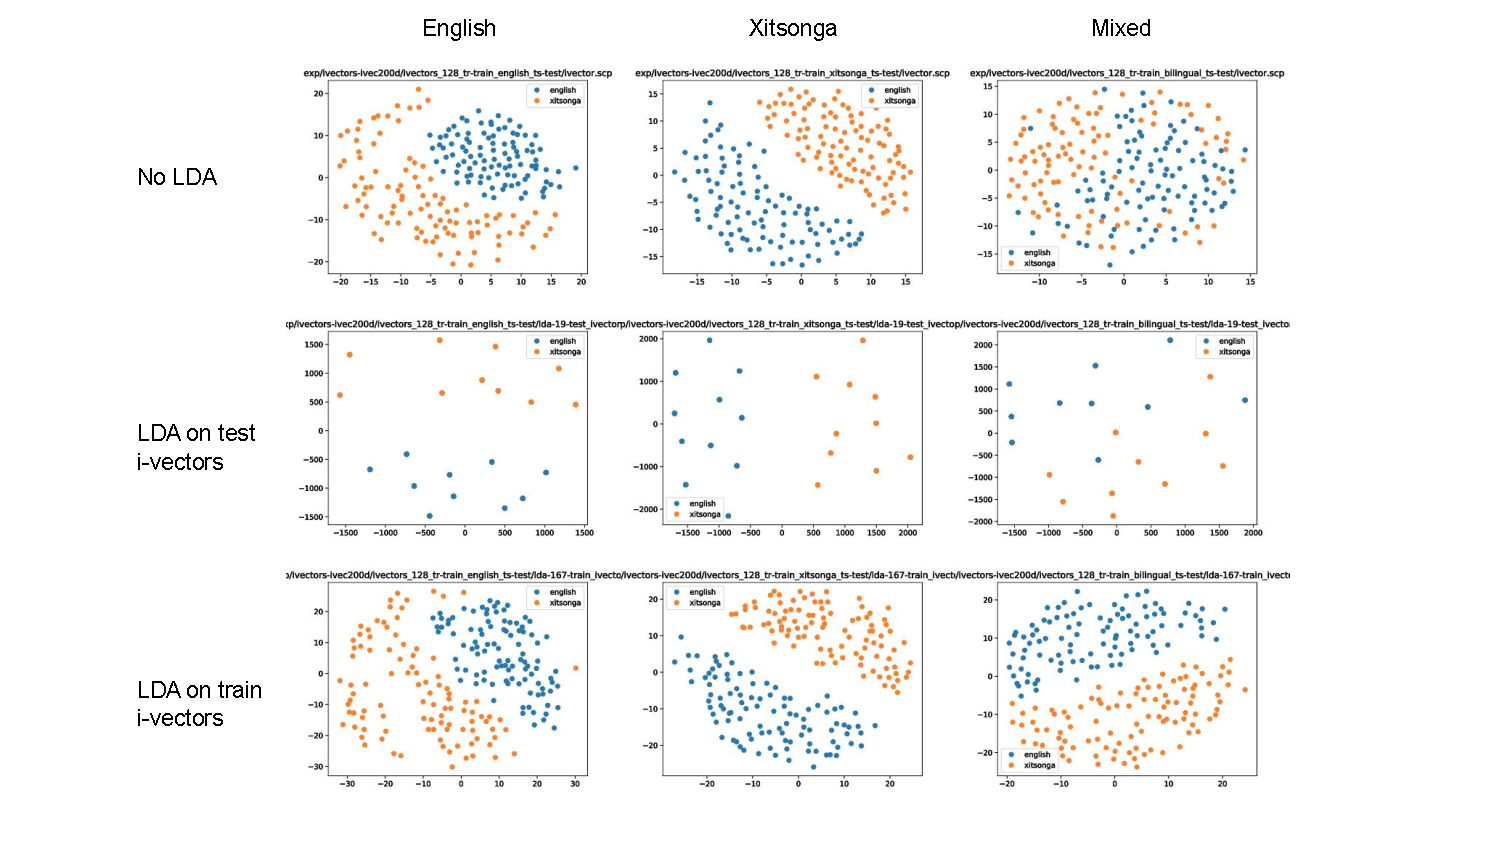
\includegraphics[width=\textwidth, height=\textheight,keepaspectratio,trim={1.5cm 0cm 1.5cm 0cm},clip]{julia_mds_replic_lda.pdf}}
\caption{Multidimensional Scaling plot of English (blue) and Xitsonga (orange) test utterances for three different language backgrounds (English, Xitsonga and Mixed), pre-LDA, post-LDA on test i-vectors  and post-LDA on train i-vectors (top, middle and bottom rows respectively); for the replication results of \citet{carbajal2016language} experiment.}
\label{Figure: Julia Replication MDS - lda}
\end{figure}


% Please add the following required packages to your document preamble:
% \usepackage{multirow}
\begin{table}[h!]
\centering
\begin{tabular}{lccc}
\hline
\multirow{2}{*}{Background} & \multicolumn{3}{c}{ABX score} \\
 & pre-LDA & \begin{tabular}[c]{@{}c@{}}post-LDA\\ (on test i-vectors)\end{tabular} & \begin{tabular}[c]{@{}c@{}}post-LDA\\ (on train i-vectors)\end{tabular} \\ \hline
English & 76.2 \textit{(73.8)} & 99.7 \textit{(98.6)} & 72.9 \textit{(70.2}) \\
Xitsonga & 79.6 \textit{(77.7)} & 97.7 \textit{(98.0)} & 79.4 \textit{(77.4)} \\
Mixed & 64.9 \textit{(61.5)} & 75.0 \textit{(72.5)} & 89.5 \textit{(88.4)} \\ \hline
\end{tabular}
\caption{Summary of ABX results (in \% correct) in the replication of \citet{carbajal2016language}'s experiment, with an i-vector dim of 200. The abx scores in italics as those obtained when excluding with the same speaker in the within-class pair. }
\label{Table: ABX score Julia Exp - lda}
\end{table}


\bigskip
%key points
\par \noindent \fbox{\parbox{\textwidth}{
\begin{itemize}[leftmargin=*]
    \setlength\itemsep{0em}
    %\renewcommand\labelitemi{$\circ$}
    \item \textbf{Modified i-vector dimension (200) to allow \acrshort{lda} on train i-vectors.}
    \item \textbf{Similar patterns as in Section \ref{Section: julia rep results} observed with increased dimension.}
    \item \textbf{In post-\acrshort{lda} \acrshort{mds} plots, seem that only one point per speaker, possibly because the larger dimension captured nearly perfectly the speakers' utterances representations.}
    \item \textbf{No significant effect of train-based \acrshort{lda} on monolingual training backgrounds.}
    \item\textbf{Train-based \acrshort{lda} significantly improves the scores in the mixed training condition.}
\end{itemize}}}



%%%%%%%%%%%%%%%%%%%%%%%%%%%%%%%%%%%%%%%%%%%%%%%%%%%%%%%%%%%%
\subsection{Effect of dynamic features} \label{Section: julia rep dynamic}
\citet{carbajal2016language} suggested that capturing dynamic information as well as the static ones could potentially enhance language separation. This is what is tested in this Section, where \acrfull{sdc} are added along with the original \acrshort{mfcc}s. 
Other than these additional coefficients, the set up is the same as in Section \ref{Section: Julia rep exp - lda} - with 200 dimensions i-vectors.
\bigskip
\par \noindent Results are presented in Table \ref{Table: ABX score Julia Exp - lda - dynamic} and Figure \ref{Figure: Julia Replication MDS - dynamix}. There doesn't seem to be any noticeable difference in the abx scores and \acrshort{mds} plots compared to those in Section \ref{Section: Julia rep exp - lda} when the background is monolingual, regardless of whether \acrshort{lda} is applied.
\par There is however significant differences when using dynamic features when the background is mixed the abx scores being higher with the dynamic features. This effect is even more salient after \acrshort{lda}. This can also be seen, in the post-\acrshort{lda} case, on the \acrshort{mds} plot, where the separation between both languages is really salient.  
\par These results could be explained by the fact that Xitsonga and English are two extremely different languages in terms of rhythm and prosody. If the background is mixed, the dynamic differences could thus be considered relevant and captured in the i-vector dimensions, whereas this wouldn't be captured with a monolingual training background.


% Please add the following required packages to your document preamble:
% \usepackage{multirow}
\begin{table}[h!]
\bigskip %?
\centering
\begin{tabular}{lccc}
\hline
\multirow{2}{*}{Background} & \multicolumn{3}{c}{ABX score} \\
 & pre-LDA & \begin{tabular}[c]{@{}c@{}}post-LDA\\ (on test i-vectors)\end{tabular} & \begin{tabular}[c]{@{}c@{}}post-LDA\\ (on train i-vectors)\end{tabular} \\ \hline
English & 75.9 \textit{(73.8)} & 96.4 \textit{(96.0)} & 70.7 \textit{(67.8)} \\
Xitsonga & 78.0 \textit{(76.1)} & 99.8 \textit{(99.8)} & 78.3 \textit{(76.1)} \\
Mixed & 68.2 \textit{(65.2)} & 92.5 \textit{(91.7)} & 99.5 \textit{(99.5)} \\ \hline
\end{tabular}
\caption{Summary of ABX results (in \% correct) in the replication of \citet{carbajal2016language}'s experiment, with an i-vector dim of 200, and additional SDC features. The abx scores in italics as those obtained when excluding with the same speaker in the within-class pair. }
\label{Table: ABX score Julia Exp - lda - dynamic}
\end{table}

\begin{figure}[h!]
\bigskip %?
\fbox{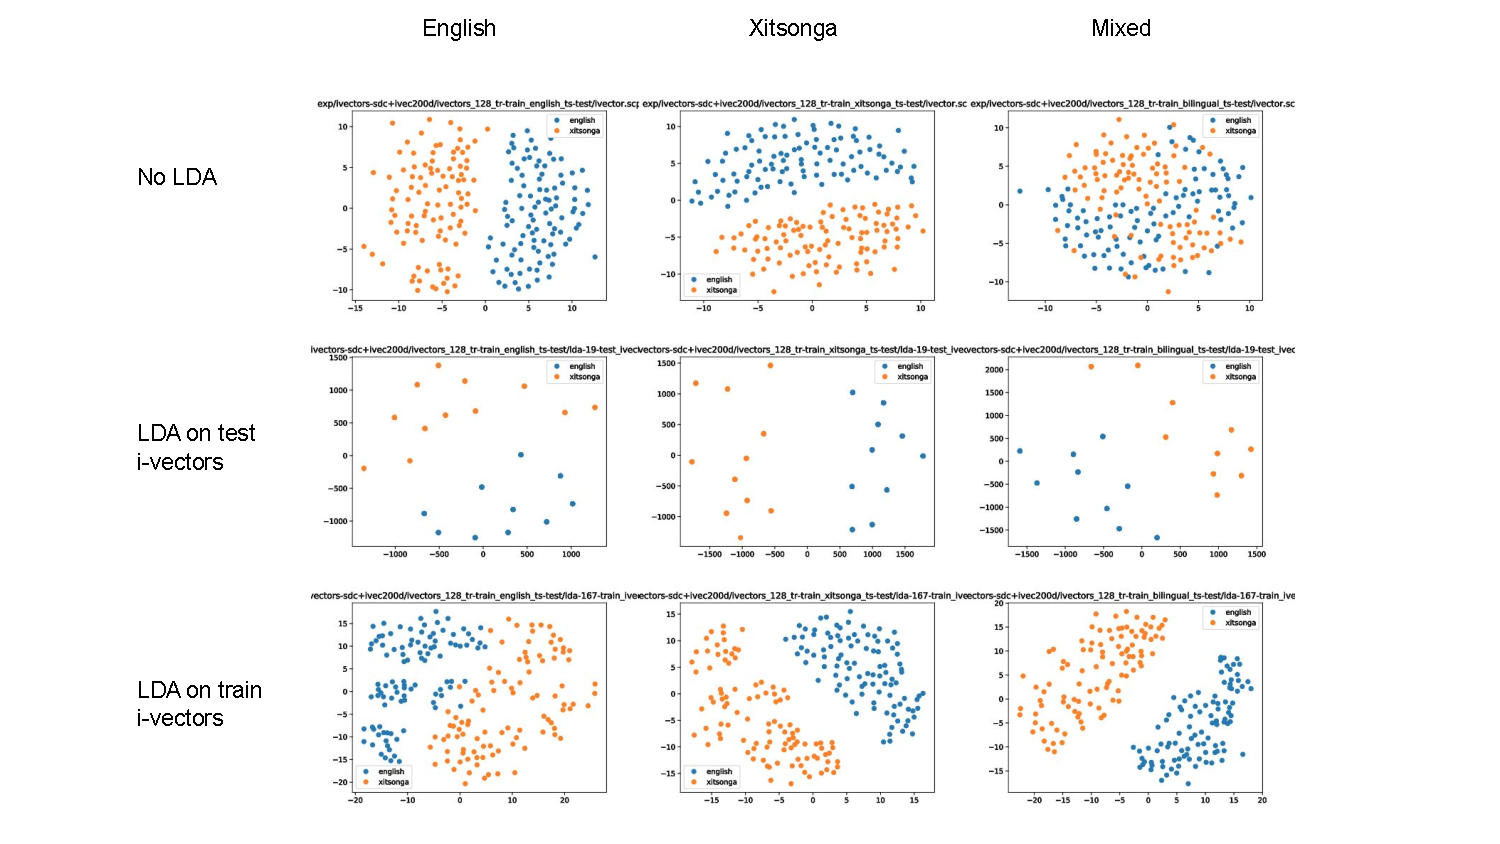
\includegraphics[width=\textwidth, height=\textheight,keepaspectratio,trim={1.5cm 0cm 1.5cm 0cm},clip]{julia_mds_replic_lda_dynamic.pdf}}
\caption{Multidimensional Scaling plot of English (blue) and Xitsonga (orange) test utterances for three different language backgrounds (English, Xitsonga and Mixed), pre-LDA, post-LDA on test i-vectors  and post-LDA on train i-vectors (top, middle and bottom rows respectively); for the replication results of \citet{carbajal2016language} experiment. The difference with Figure \ref{Figure: Julia Replication MDS - lda} is that \acrshort{sdc} are added to the features.}
\label{Figure: Julia Replication MDS - dynamix}
\end{figure}

\bigskip
%key points
\par \noindent \fbox{\parbox{\textwidth}{
\begin{itemize}[leftmargin=*]
    \setlength\itemsep{0em}
    %\renewcommand\labelitemi{$\circ$}
    \item \textbf{Same setup as in Section \ref{Section: Julia rep exp - lda}}
    \item \textbf{Significant effect of dynamic features on the mixed training condition only}
    \item \textbf{Suggest that when mixed training, the dynamic features are considered relevant - as very different rythm and prosody between the two languages.}
\end{itemize}}}


%%%%%%%%%%%%%%%%%%%%%%%%%%%%%%%%%%%%%%%%%%%%%%%%%%%%%%%%%%%%
\subsection{Discussion}

\todo{to fill in + transition for next section.}



%###########################################################
%###########################################################
\section{Impact of bilingual environment in LID}\label{Section: Impact bilingual env}
%###########################################################
%###########################################################

In this Section, we investigate further the effect of bilingualism in \acrshort{lid}. Specifically, we look into bilingualism in training when speakers are themselves bilingual, and speak both languages. This differs to the mixed design in Section \ref{Section: impact of multilingual in lid} where speakers only speak one of the two languages. This new design could correspond, in real-life settings, to children being raised in and exposed to fully bilingual environments, where their relatives switch between at least two languages. Such a setup could give us hints on the advantages of \textit{practising} - or not - code-switching around children; although it is definitely not enough to make causal relationships. 


% replicating CArbajal experiment with EMIME dataset 

%%%%%%%%%%%%%%%%%%%%%%%%%%%%%%%%%%%%%%%%%%%%%%%%%%%%%%%%%%%%
\subsection{Theoretical questions}

\begin{itemize}
    \renewcommand\labelitemi{--}
    \item showed that i-vectors good model of \acrshort{lid}
    \item investigate further impact of bilingualism
    \item role of speaker - when not possible to use speaker identity to do lid. 
    \item link with cognitive approaches.
    \item less speakers - closer to ecological. 
    \item NEED TO FIND EXPERIMENTAL PAPERS?
\end{itemize}


\subsection{Methods}


In this Section, the \acrshort{emime} dataset is used, as it contains bilingual speakers. Refer to Section \ref{Section: emime dataset} for more details.
\bigskip
\par \noindent The pipeline is the same as the one described in Section \ref{Section: replication pipeline}, with additional dynamic coefficients - as done in Section \ref{Section: julia rep dynamic}. When \acrshort{lda} is mentioned, it refers to \acrshort{lda} carried out on the train set, except explicitly mentioned. Because the \acrshort{emime} dataset contains less speakers than the \acrshort{ex} one, we kept the original i-vector dimensions of 150. \textit{(Means that can't exactly compare to Sections \ref{Section: Julia rep exp - lda} and \ref{Section: julia rep dynamic}?)}


%%%%%%%%%%%%%%%%%%%%%%%%%%%%%%%%%%%%%%%%%%%%%%%%%%%%%%%%%%%%
\subsection{Preliminary Results}


\begin{itemize}
    \renewcommand\labelitemi{--}
    \item less speakers - closer to ecological. 
    \item look into abx per speakers. 
    \item Report problem of sentence repetitions. Very important. 
    \item Suggest that results when filterd out are terrible?????? WHY

\end{itemize}


 \par \noindent We present different kind of results. The "filtered" results correspond to the results in italics in Tables \ref{Table: ABX score Julia Rep}, \ref{Table: ABX score Julia Exp - lda} and \ref{Table: ABX score Julia Exp - lda - dynamic}. However, they can only be used when there is no bilingual speaker (ie with the ``mono'' test set). We could have modified to filter to account for this specific situation, ensuring that no speaker is the same in any of the item from the triplet (which was already the case in \ref{Section: impact of multilingual in lid} as the between-class items cound't have the same speaker - by design). However it would mean the abx scores wouldn't be weighed, as there'd be different numbers of triplets one way than the other, and even using weighed average scores, it wouldn't be as meaningful. Other ways to measure abx scores when there are abx speakers is to use the ``across" option flag, discarding the speaker bias by forcing the two "between items" to have the same speaker, itself different from the "goal" item X. \textbf{The only scores which can be compared are thus the raw ones - albeit not right measure? No can't compare anyway cause different test sets so different utterances obvs. }% DOESNT MAKE ANY SENSE TO USE OUR FILTERED MEASURE HERE AS IT ONLY ENSURES THAT  A AND X ARE DIFFERENT BUT A COULD BE EQUAL TO B

We can't compare the effect on the test sets as not same utterances. 

\bigskip
\par Really low scores (When mono set) means that they take only speaker info???
Also add by speaker table for bil test. 
Table ABX Filtered test bilingual . Also ADD per speaker in parenthesis for test 




% Please add the following required packages to your document preamble:
% \usepackage{booktabs}
% \usepackage{multirow}
\begin{table}[h!]
\centering
\begin{tabular}{@{}llll@{}}
\toprule
\multirow{2}{*}{Test set (mono)} & \multirow{2}{*}{Background} & \multicolumn{2}{c}{ABX score} \\ \cline{3-4}
 &  & \multicolumn{1}{c}{pre-LDA} & \multicolumn{1}{c}{post-LDA} \\ \midrule
\multirow{5}{*}{English - Finnish} & English Native & 66.1 (38.0) & \textbf{62.8} \textbf{\textit{(28.2)}} \\
 & English & \textbf{75.1} \textbf{\textit{(53.1)}} & 56.1 \textit{(13.2)} \\
 & Finnish & 71.1 \textit{(45.3)} & 57.3 \textit{(16.2)} \\
 & Mixed & 71.5 \textit{(46.5)} & 58.8 \textit{(18.6)} \\
 & Bilingual & 70.6 \textit{(44.8)} & 56.5 \textit{(14.2)} \\ \midrule
\multirow{5}{*}{English - German} & English Native & 76.2 \textit{(54.8)} & 61.2 \textit{(28.5)} \\
 & English & 74.0 \textit{(50.9)} & 64.5 \textbf{\textit{(31.2)}} \\
 & German & 73.8 \textit{(54.2)} & \textbf{64.8} \textit{(30.5)} \\
 & Mixed & \textbf{83.2} \textbf{\textit{(68.6)}} & 63.7 \textit{(28.7)} \\
 & Bilingual & 73.5 \textit{(52.6)} & 65.7 \textit{(32.3)} \\ \bottomrule
\end{tabular}
\caption{Summary of ABX results (in \% correct) in the EMIME experiment for the different mono test sets.  Additional SDC features. The abx scores in brackets are \textbf{those obtained when excluding with the same speaker in the within-class pair}. }
\label{Table: xxx}
\end{table}







% Please add the following required packages to your document preamble:
% \usepackage{booktabs}
% \usepackage{multirow}
\begin{table}[]
\centering
\begin{tabular}{@{}llcc@{}}
\toprule
\multirow{2}{*}{Test set (bil)} & \multirow{2}{*}{Background} & \multicolumn{2}{c}{ABX score} \\  \cline{3-4}
 &  & pre-LDA & post-LDA \\ \midrule
\multirow{5}{*}{English - Finnish} & English Native & 58.7 (58.3) & 57.6 (54.2) \\
 & English & 58.3 \textit{(60.9)} & 56.3 \textit{(50.3)} \\
 & Finnish & \textbf{62.6} \textbf{\textit{(70.6)}} & 54.7 \textit{(48.6)} \\
 & Mixed & 62.2 \textit{(69.9)} & \textbf{60.4} \textbf{\textit{(56.4)}} \\
 & Bilingual & 60.0 \textit{(64.0)} & 54.8 \textit{(49.0)} \\ \midrule
\multirow{5}{*}{English - German} & English Native & 55.7 \textit{(56.4)} & 55.9 \textit{(53.2)} \\
 & English & 56.9 \textit{(57.6)} & 54.7 \textit{(54.1)} \\
 & German & 55.3 \textit{(53.2)} & 54.9 \textit{(53.4)} \\
 & Mixed & \textbf{58.3} \textbf{\textit{(59.4)}} & \textbf{58.4} \textbf{\textit{(57.6)}} \\
 & Bilingual & 56.9 \textit{(53.8)} & 55.2 \textit{(56.2)} \\ \bottomrule
\end{tabular}
\caption{Summary of ABX results (in \% correct) in the EMIME experiment for the different bilingual test sets.  Additional SDC features. The abx scores in brackets are the \textbf{across speaker} ones \textit{(Careful - different of those in the mono test set table - put reference)}. }
\label{Table: xxx}
\end{table}

\textbf{NEED FIGURES WITH SDC ABSOLUTELY. }
%%%%%%%%%%%%%%%%%%%%%%%%%%%%%%%%%%%%%%%%%%%%%%%%%%%%%%%%%%%%
\subsection{Role of Speaker Information}

- look into ABX per speaker

\begin{table}[]
\begin{tabular}{lcc}
\hline
Background & \multicolumn{2}{c}{ABX score} \\
 & pre-lda & post-lda (train) \\ \hline
English Native & 70.7 & 63.3 \\
English & 65.1 & 69.2 \\
German & 60.4 & 70.0 \\
Mixed & 68.0 & 79.0 \\
Bilingual & 64.7 & 65.1 \\ \hline
\end{tabular}
\caption{BY speaker. With SDC. English - German}
\end{table}




%###########################################################
%###########################################################
\section{Using ecological data in \acrshort{lid}}
%###########################################################
%###########################################################

% Use more ecological data to see how it works in real life. We never have as clean datasets ("mixed" - "bilingual"), it's usually a bit of some vlanguages, a bit of other, never 50/50 , + code switching within sentence. 
